\documentclass[ro]{problem}
\usepackage{tikz}
\title{Foc}

\contest{Concursul Interjudeţean Info-Oltenia 2023}
\location{România}
\date{26}{2}{2023}
\logo{info2023.jpeg}

\begin{document}

\maketitle

Satul Binăreni se află în pericol în urma incendiilor provocate în ultima lună. Acesta este reprezentat printr-o matrice binară cu $N$ linii și $M$ coloane. Toate celulele care au luat foc sunt reprezentate prin valoarea $0$. Toate celulele în care nu este produs un incendiu, reprezentate prin valori de $1$, conțin, inițial, câte o casă a unui sătean.

\par

O celulă este considerată $"safe"$ dacă nu a luat foc și se află într-una din cele două situații de mai jos:
\begin{enumerate}
    \item se află la marginea satului (pe linia $1$, respectiv $N$ sau pe coloana $1$, respectiv $M$ a matricei);
    \item cel puțin una din cele 4 celule vecine pe direcțiile $N$, $V$, $S$ și $E$ sunt $"safe"$.
\end{enumerate}

\par

Gosu, cel mai renumit pompier din sat, își dorește să salveze toate casele care nu se află în celule $"safe"$, folosindu-și superputerea: acesta poate stinge o singură dată focul din toate celulele care au luat foc pe o linie $x$ și toate celulele care au luat foc pe o coloană $y$, plasându-se la intersecția acestora, în celula $(x, y)$. Acesta se poate plasa atât pe o celulă cu incendiu, cât și pe o celulă care conține o casă. Astfel, după utilizarea superputerii sale, toate elementele de pe linia $x$, respectiv elementele de pe coloana $y$ vor căpăta valoarea $1$.

\section{Cerinţă}
Având în vedere că Gosu își poate folosi superputerea o singură dată, aflați toate perechile de coordonate $(x, y)$ posibile pe care se poate plasa acesta, astfel încât să salveze toate casele care sunt în pericol.
 
\section{Date intrare}

Pe prima linie a fișierului de intrare se găsesc două numere întregi $N$ și $M$, separate printr-un spațiu, reprezentând dimensiunile matricei.

Pe următoarele $N$ linii se află câte $M$ valori de $0$ sau $1$, separate prin spații, reprezentând descrierea matricei satului.

\section{Date ieşire}

În fișierul de ieșire se vor afișa, pe linii diferite și separate printr-un spațiu, coordonatele celulelor pe care se poate plasa Gosu pentru a salva toate casele. Perechile de coordonate vor fi afișate în ordine lexicografică. Dacă nu există o soluție, se va afișa -1. 

\begin{restrictions}
[
    \item $3\leq N, M \leq 10^3$
    \item $A_{ij} \in \{0, 1\}$, $1 \leq i \leq N$, $1 \leq j \leq M$
    \item Se garantează că există cel puțin o casă care se află în pericol.
]
\restr{30}{$1 \leq N, M \leq 10^2$}
\restr{70}{fără\ alte\ restricţii}

\end{restrictions}

\begin{examples}
\exmp{7 8
0 0 0 0 1 1 0 0
0 1 0 0 0 0 0 0
0 0 0 0 0 0 0 1
0 0 0 0 0 0 0 1
0 0 0 1 0 0 0 1
0 0 0 0 0 0 1 0
1 0 0 0 0 0 0 0
}{5 1
5 2
5 3
6 1
6 2
6 3
7 3}%
\exmp{9 9
0 0 0 0 0 0 1 0 1
0 1 0 0 0 0 0 0 0
0 0 0 0 0 0 0 0 1
0 0 0 0 0 0 0 0 1
0 0 0 0 1 0 0 0 1
0 0 0 0 0 0 0 0 1
1 0 0 0 0 0 0 0 0
0 0 0 0 0 0 0 1 0
0 0 0 0 0 0 0 0 0
}{-1}%
\end{examples}

\section{Explicație}

În primul exemplu, satul este alcătuit din $9$ case, dintre care doar $6$ sunt $"safe"$. Casele aflate în pericol sunt situate pe celulele $(2, 2)$, $(5, 4)$, respectiv $(6, 7)$. Soluția conține 7 perechi de coordonate, afișate în ordine lexicografică. Dacă alege, spre exemplu, celula $(5, 1)$, Gosu va stinge focul în: 
\begin{itemize}
    \item celula vecină din $V$ a casei din celula $(2, 2)$;
    \item celulele vecine din $V$, respectiv $E$ ale casei situate pe $(5, 4)$;
    \item celula vecină din $N$ a ultimei case.
\end{itemize}
Toți acești vecini devin, la rândul lor, $"safe"$.

\par

Pe linia $7$ există o singură celulă din care Gosu poate stinge focul în cel puțin una din celulele vecine ale fiecărei case aflate în pericol: $(7, 3)$. După folosirea superputerii sale din această celulă, matricea devine:
\begin{center}
    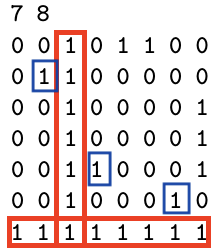
\includegraphics{foc-exemplu.png}
\end{center}

\par

În cazul celui de-al doilea exemplu, există $3$ case aflate în pericol, în celulele $(2, 2)$, $(5, 5)$, respectiv $(8, 8)$. Nu există nicio pereche de coordonate pe care Gosu se poate plasa, astfel încât să salveze toate cele $3$ case.

\end{document}